\documentclass[a4paper,12pt]{article}
\usepackage[indonesian]{babel}
\usepackage{graphicx}
\usepackage{multirow}
\usepackage{enumitem}
\usepackage{listings}
\usepackage{wrapfig}
\usepackage[T1]{fontenc}
\usepackage{inconsolata}
\usepackage{lipsum}
\usepackage{adjustbox}


\usepackage{color}
\usepackage[table,xcdraw]{xcolor}
\definecolor{mygreen}{rgb}{0,0.6,0}
\definecolor{mygray}{rgb}{0.5,0.5,0.5}
\definecolor{mymauve}{rgb}{0.58,0,0.82}
\lstset{%
    language=java,
    showstringspaces=false,          % Prevent tex replacing space to bracket in code
    frame=single,                    % Set frame around code
    backgroundcolor=\color{white},   % choose the background color
    basicstyle=\footnotesize,        % size of fonts used for the code
    breaklines=true,                 % automatic line breaking only at whitespace
    captionpos=b,                    % sets the caption-position to bottom
    commentstyle=\color{mygreen},    % comment style
    keywordstyle=\color{blue},       % keyword style
    stringstyle=\color{mymauve},     % string literal style
    numbers=left,
}

\graphicspath{ {./img/} }
\begin{document}
\title{ {\Large Laporan Praktikum}\\ Analisis dan Desain Sistem\\{\Large Pertemuan 2}}

\author{Aldzikri Dwijayanto Prathama
    \\195410189
    \\Informatika}
\makeatletter
\begin{titlepage}
    \begin{center}
        {\huge \bfseries \@title}\\[14ex]
        
\includegraphics[scale=.8]{logo}\\[4ex]
        {\large \@author}\\[12ex]
        {\large \bfseries {SEKOLAH TINGGI MANAJEMEN INFORMATIKA DAN KOMPUTER
            AKAKOM YOGYAKARTA}}
    \end{center}


%{\large \@date}
\end{titlepage}
\makeatother
%\maketitle
\newpage
\tableofcontents
\newpage

\section{Tujuan}
Mahasiswa mampu:
\begin{enumerate}
   \item menjelaskan proses bisnis yang ada dalam sebuah sistem
   \item Membuat analisis sistem sesuai dengan langkah-langkah yang ditetapkan
\end{enumerate}

\section{Dasar Teori}
Analisis Sistem adalah penguraian dari suatu sistem informasi yang utuh ke dalam bagian-bagian komponennya
dengan maksud untuk mengidentifikasikan dan mengevaluasi permasalahan-permasalahan, kesempatan-kesempatan,
hambatan-hambatan yang terjadi dan kebutuhan-kebutuhan yang diharapkan sehingga dapat diusulkan
perbaikan-perbaikannya. Hasil dari suatu analisis sistem adalah kebutuhan sistem yang akan digunakan untuk
melakukan desain sistem. Langkah dalam analisis sistem :
\begin{enumerate}
    \item Studi kelayakan, meliputi:
        \begin{enumerate}[label=\alph*.]
            \item Penentuan masalah
            \item Pembentukan sasaran sistem
            \item Pengidentifikasian pemakai sistem
            \item Pembentukan lingkup sistem
        \end{enumerate}
    \item Analisis kebutuhan:
        \begin{enumerate}[label=\alph*.] 
            \item Masukkan yang diperlukan sistem
            \item Keluaran yang dibutuhkan
            \item Lingkup proses
            \item Volume data yang ditangani sistem
            \item Kategori pemakai sistem
            \item Kontrol sistem
        \end{enumerate}
\end{enumerate}

\newpage

\section{Pembahasan}
\subsection{Praktik}
Diberikan deskripsi sebagai berikut:\\
Sebuah usaha tour “CAHAYA TOUR” yang masih sederhana selalu kewalahan melayani
konsumen yang bertanya mengenai info wisata yang bisa dikunjungi dan biayanya. Pemilik “CAHAYA TOUR” sedang  berpikir
bagaimana  memanfaatkan teknologi informasi untuk mendukung usaha tour yang dimiliki sehingga memudahkan para
konsumen mendapatkan informasi dan meningkatkan layanan “CAHAYA TOUR” terhadap para konsumen. \\
Lakukan analisis sistem untuk kasus di atas!

\subsubsection{Studi Kelayakan}
\begin{center}
    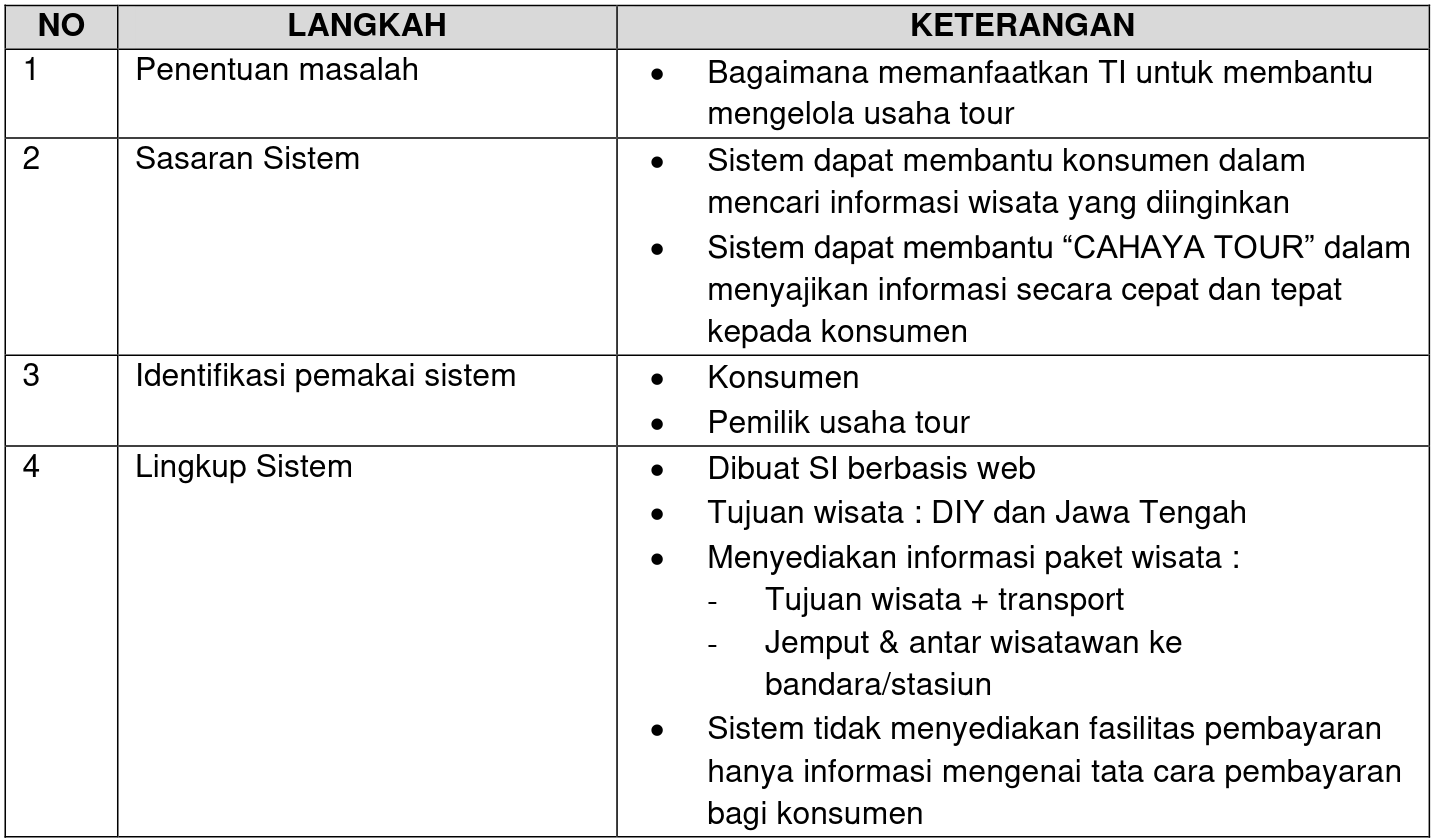
\includegraphics[width=\textwidth]{tabel1.png} 
\end{center}
\paragraph*{Pembahasan\\}
Dari deskripsi masalah diatas, diketahui pemilik usaha tour ingin memanfaatkan teknologi informasi, untuk
membantu usahanya melayani konsumen.
\begin{enumerate}
    \item Penentuan masalah\\
        Langkah pertama adalah menentukan masalah yang akan diselesaikan sistem. Sistem yang dibangun harus bisa
        menyelesaikan masalah yang harus diselesaikan, yaitu untuk menyediakan informasi kepada konsumen.

    \item Sasaran sistem\\
        Sasaran utama dari sistem yang akan dibuat, pada kasus ini sasaran utama sistem yang dibangun adalah
        membantu konsumen mencari informasi wisata, dan menyajikan informasi secara cepat dan tepat.

    \item Identifikasi pemakaian sistem\\
        Mengidentifikasi, siapa saja yang akan menggunakan sistem yang akan dibangun.

    \item Langkah lingkup sistem\\
        Merupakan deskripsi dan spesifikasi kasar, tentang sistem yang akan dibangun.
\end{enumerate}

\subsection{Latihan}
    Latihan terlampir

\newpage
\subsection{Tugas}
Akan dibangun sebuah sistem informasi yang dapat membantu pengelolaan pendaftaran asisten laboratorium. Sistem ini
direncanakan berbasis web. Asisten praktikum di lab. dibutuhkan untuk membantu dosen dalam pelaksanaan kegiatan
praktikum.\\
Mekanismenya
\begin{enumerate}
   \item Calon asisten:
       \begin{itemize}
          \item Mengisi form pendaftaran menjadai asisten lab (download) 
          \item Mengumpulkan form pendaftaran yg sdh diisi disertai 
              \begin{enumerate}[label=\alph*.]
                  \item Foto 4x6
                  \item Transkrip nilai
              \end{enumerate}
         \item Calon asistem menunggu pengumuman penerimaan menjadi asisten
       \end{itemize}
    
    \item Administrasi laboratorium:
        \begin{itemize}
           \item Memasukkan data praktikum yang membutuhkan asisten beserta jadwalnya
           \item Menyeleksi asisten yang mendaftar
           \item Mengumumkan calon asisten yang diterima sebagai asisten
        \end{itemize}
\end{enumerate}

Sistem yang akan dibuat nantinya:
\begin{enumerate}[label=\alph*.]
   \item Menyediakan form pendaftaran asisten di web dan dapat di unduh
   \item Menampilkan daftar mata praktikum beserta jadwalnya yang membutuhkan praktikum
   \item Menampilkan pengumuman calon asisten yang diterima menjadi asisten lab.
\end{enumerate}
\paragraph*{Analisis kebutuhan\\}

\begin{table}[!h]
\begin{tabular}{|c|l|l|}
\hline
\rowcolor[HTML]{C0C0C0} 
    \textbf{No} & \multicolumn{1}{c|}{\cellcolor[HTML]{C0C0C0}\textbf{Langkah}} &
    \multicolumn{1}{c|}{\cellcolor[HTML]{C0C0C0}\textbf{Keterangan}} \\ \hline
1 & \begin{tabular}[c]{@{}l@{}}Masukan yang diperlukan \\ system\end{tabular} & \begin{tabular}[c]{@{}l@{}}NIM\\ Nama\\ Jurusan\\ Email\\ Foto 4x6\\ Transkrip nilai\end{tabular} \\ \hline
2 & Keluaran yang dibutuhkan & \begin{tabular}[c]{@{}l@{}}Form pendaftaran\\ Data diri mahasiswa\\ Daftar dan jadwal praktikum\\ Pengumuman\end{tabular} \\ \hline
3 & Lingkup Proses & \begin{tabular}[c]{@{}l@{}}Halaman pendaftaran\\ Memilih praktikum\\ Seleksi\\ Pengumuman\end{tabular} \\ \hline
4 & \begin{tabular}[c]{@{}l@{}}Volume data yang ditangani \\ system\end{tabular} & \begin{tabular}[c]{@{}l@{}}Data mahasiswa pendaftar\\ Foto mahasiswa pendaftar\end{tabular} \\ \hline
5 & Kategori pemakaian system & \begin{tabular}[c]{@{}l@{}}Administrasi lab\\ Mahasiswa\end{tabular} \\ \hline
6 & Kontrol system & \begin{tabular}[c]{@{}l@{}}Mahasiswa dapat memasukkan form\\ Administrasi sebagai admin sistem\end{tabular} \\ \hline
\end{tabular}
\end{table}
\paragraph*{Pembahasan\\}
Pada input sistem pendaftaran, sistem akan menerima input berupa data diri mahasiswa, foto, dan transkrip nilai yang
nantinya akan disimpan ke sistem.\\

Keluaran yang akan dihasilkan sistem pendaftaran kepada administrasi laboratorium diantaranya data diri mahasiswa.
Sedangkan Keluaran yang diberikan kepada mahasiswa pendaftar diantaranya form pendaftaran, daftar dan jadwal praktikum,
serta pengumuman.\\

Langkah proses yang ada pada sistem adalah halam pendaftaran sebagai tempat mahasiswa memasukkan data diri, kemudian
memilih mata kuliah praktikum. Setelah itu administrasi lab akan melakukan seleksi, dan sistem akan menampilkan
pengumuman.\\

Volume data, data yang akan disimpan oleh sistem adalah form pendaftaran mahasiswa, dan foto mahasiswa.\\

Kategori pemakai sistem adalah administrasi lab, dan mahasiswa pendaftar.\\

Kontrol sistem, administrasi lab bertindak sebagai admin sistem, dan mahasiswa sebagai user.

\section{Kesimpulan}
Setelah praktik mahasiswa mampu menjelaskan proses bisnis yang ada dalam sebuah sistem, dan membuat analisis sistem
sesuai dengan langkah-langkah yang ditetapkan.
    
\end{document}
